\section{Durchführung}
\label{sec:Durchführung}

Der verwendete Versuchsaufbau ist in \autoref{fig:aufbau} schematisch dargestellt.

\begin{figure}
    \centering
    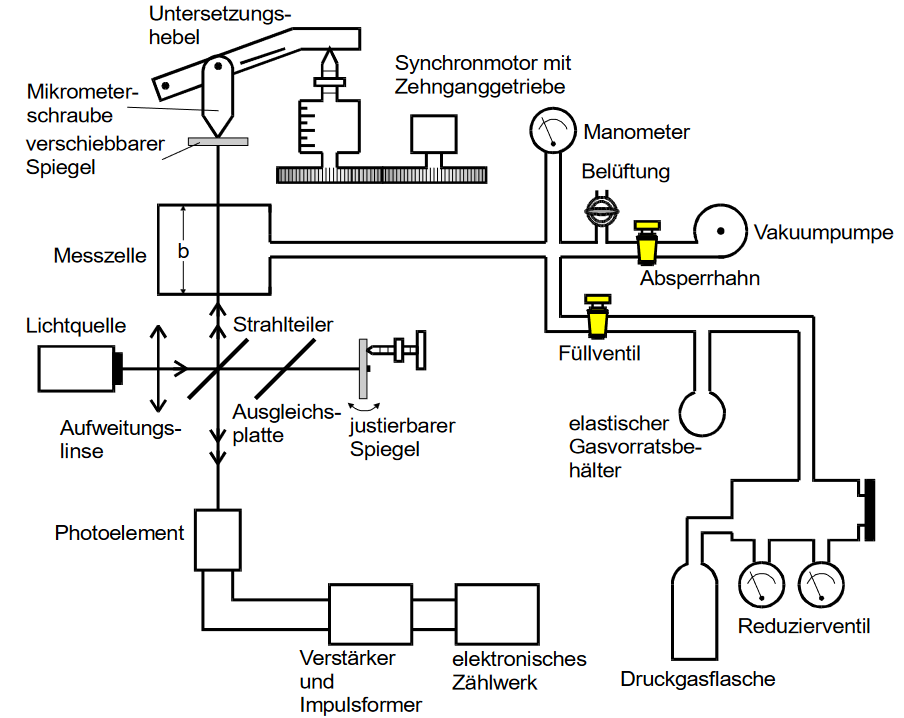
\includegraphics{content/aufbau.png}
    \caption{Schematische Darstellung der verwendeten Messapparatur.}
    \label{fig:aufbau}
  \end{figure}

Kern des Aufbaus ist ein Michelson-Interferometer, dessen Funktionsweise in \autoref{sec:theorie} beschrieben ist.
Der Detektor ist an ein elektronisches Zählwerk angeschlossen, wobei ein Verstärker und Impulsformer zwischen Detektor und 
Zählwerk geschaltet ist. Dieser Aufbau erlaubt das Registrieren und Zählen der am Detektor durchlaufenden Interferenzmaxima. 
Zwischen Strahlteiler und verschiebbarem Spiegel ist zudem eine Messzelle verbaut. Der Druck in ihrem Inneren kann mit Hilfe
einer Handpumpe variiert werden. 
Vor Beginn der Versuchsdurchführung muss eine Justierung des Interferometers erfolgen. Es ist dabei sicherzustellen,
dass die von den Spiegeln $S1$ und $S2$ eintreffenden Strahlenbündel parallel zueinander auf den Detektor treffen. 
Die Apparatur wird mit Hilfe der Stellschrauben an den Spiegeln so justiert, dass die beiden hellsten Lichtpunkte 
auf dem Detektor möglichst gut zur Deckung kommen. 

Nach abgeschlossener Justierung kann das Interferometer zur Wellenlängenmessung des verwendeten Lasers genutzt werden. 
Dazu wird der verschiebbare Spiegel mit einem Synchronmotor und einer Mikrometerschraube mit konstanter Geschwindigkeit 
verschoben. Diese Geschwindigkeit darf jedoch nicht zu hoch gewählt werden, muss darauf geachtet werden, da das Photoelement 
ansosnten nicht alle Impulse ausreichend erkennen und aufzeichnen kann. Es wird jeweils eine Spiegelverschiebung von 
$d \approx \SI{5}{\milli\meter}$ durchgeführt und jeweils die vom Photoelement registrierten Interferenzmaxima notiert.
Diese Messung wird insgesamt zehn Mal durchgeführt. 

Für die Bestimmung des Brechungsindex von Luft verbleibt der verschiebbare Spiegel in einer festen Position.
Die Messzelle wird unter Verwendung der Handpumpe auf einen Druck $p$ evakuiert, welcher notiert wird. Es wird zudem die Zahl 
der Interferenzmaxima notiert, die beim Wiedereinlassen der Luft in die Messzelle aufgezeichnet werden. 
Eine solche Einzelmessung wird beendet, wenn sich in der Messzelle wieder Normaldruck eingestellt hat. 
Diese Messung wird ebenfalls zehn Mal durchgeführt. 